\chapter{Methodology}
\label{cha:4}

\section{Dataset split}

The dataset reliability scores are grouped and split into 4 classes based on its reliability score as previously described in Section \ref{bat-characteristics}:
\begin{enumerate}
    \item Problematic: scores between 0.00 and 24.00
    \item Questionable: scores between 24.01 and 32.00
    \item Generally Reliable: scores between 32.01 and 40.00
    \item Reliable: scores between 40.01 and 64
\end{enumerate}

\begin{table}[htbp]
    \centering
    \begin{tabular}{| c | c | c | c |}
        \hline
        Class              & Train Set & Test Set & Validation Set \\
        \hline
        Problematic        & 287       & 27       & 34             \\
        Questionable       & 611       & 1033     & 2394           \\
        Generally Reliable & 54        & 104      & 384            \\
        Reliable           & 70        & 128      & 371            \\
        \hline
        Total              & 4325      & 569      & 603            \\
        \hline
    \end{tabular}
    \caption{Number of total samples and on each class in train, test, and validation set}
    \label{table:dataset_split}
\end{table}

The dataset is then split into three sets of train, test, and validation, distributed as can be seen in Table \ref{table:dataset_split}. The split is done in a way to ensure that articles from different outlets are distributed equally between the three sets. A major drawback of this 'balance' splitting is that there is no unseen outlet in the test set and validation set. This can influence the final test metrics and may hinder the model's ability to generalise to new, unseen articles from unseen outlets. However, considering that new outlets are rarely introduced in the real life, it might be beneficial to slightly overfit on the patterns of existing outlets.


\section{Features and baselines}

The primary features include the title and content of the articles. Ideally, a reliable article-level media bias classifier should be capable of generalising based predominantly on the content of the articles. Furthermore, outlet information may be incorporated as an additional feature in certain instances, enabling a comparative analysis of the classifier's performance with and without the inclusion of this supplementary data.

As baselines, traditional encoding methods such as Bag-of-Words and TF-IDF are implemented, combined with a simple logistic regression classifier. In these cases, the validation set is concatenated into the training set. Additionally, a majority baseline based on outlet is implemented for comparison, to demonstrate the influence of outlet information on this task. This method works by taking the most frequently occurring class observed among articles from each outlet and use it as the predicted value for the article. \textit{If an article is from outlet A, and the majority of articles from outlet A are classified as class X, then article A is classified as class X}. An illustration can be seen in Figure \ref{fig:majority_baseline}.


\begin{figure}[htbp]
    \centering
    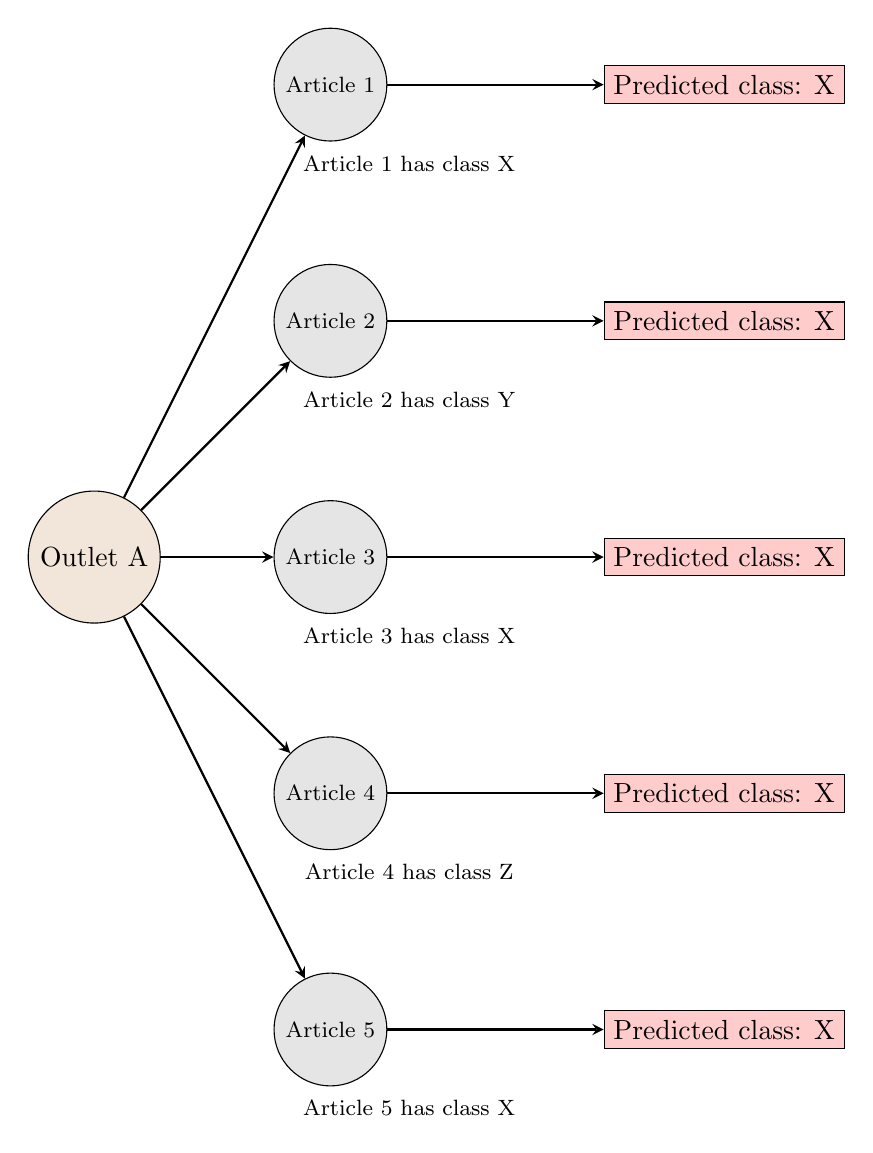
\begin{tikzpicture}
        \tikzstyle{outlet} = [circle, draw, fill=brown!20, text centered]
        \tikzstyle{prediction} = [rectangle, draw, fill=red!20, text centered]
        \tikzstyle{article} = [circle, draw, fill=gray!20, text centered, font=\footnotesize]
        \tikzstyle{arrow} = [thick,->,>=stealth]
        \tikzstyle{label} = [text centered, font=\footnotesize]

        \node[outlet] (outletA) at (0, 6) {Outlet A};

        \node[article] (A1) at (3, 12) {Article 1};
        \node[article] (A2) at (3, 9) {Article 2};
        \node[article] (A3) at (3, 6) {Article 3};
        \node[article] (A4) at (3, 3) {Article 4};
        \node[article] (A5) at (3, 0) {Article 5};

        \draw[arrow] (outletA) -- (A1);
        \draw[arrow] (outletA) -- (A2);
        \draw[arrow] (outletA) -- (A3);
        \draw[arrow] (outletA) -- (A4);
        \draw[arrow] (outletA) -- (A5);

        \node[prediction] (ClassA1) at (8, 12) {Predicted class: X};
        \node[prediction] (ClassA2) at (8, 9) {Predicted class: X};
        \node[prediction] (ClassA3) at (8, 6) {Predicted class: X};
        \node[prediction] (ClassA4) at (8, 3) {Predicted class: X};
        \node[prediction] (ClassA5) at (8, 0) {Predicted class: X};

        \draw[arrow] (A1) -- (ClassA1);
        \draw[arrow] (A2) -- (ClassA2);
        \draw[arrow] (A3) -- (ClassA3);
        \draw[arrow] (A4) -- (ClassA4);
        \draw[arrow] (A5) -- (ClassA5);

        \node[label] at (4, 11) {Article 1 has class X};
        \node[label] at (4, 8) {Article 2 has class Y};
        \node[label] at (4, 5) {Article 3 has class X};
        \node[label] at (4, 2) {Article 4 has class Z};
        \node[label] at (4, -1) {Article 5 has class X};
    \end{tikzpicture}
    \caption{Majority baseline based on outlet, every article here will be predicted as X since X is the most frequently observed class in outlet A}
    \label{fig:majority_baseline}
\end{figure}

\section{Proposed methods}

\subsection{BoW + MLP}

\begin{figure}[htbp]
    \centering
    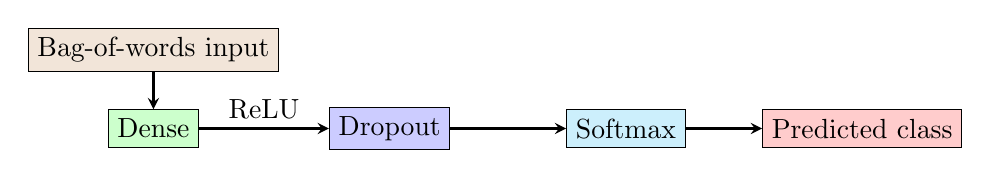
\begin{tikzpicture}
        \tikzstyle{arrow} = [thick,->,>=stealth]

        \node (input) [draw, align=center, fill=brown!20] {Bag-of-words input};
        \node (dense) [draw, below of=input, fill=green!20] {Dense};
        \draw[arrow] (input.south) -- (dense.north);
        \node (dropout) [draw, right of=dense, xshift=2cm, fill=blue!20] {Dropout};
        \draw[arrow] (dense.east) -- node[above, midway, fill=white] {ReLU} (dropout.west);
        \node (softmax) [draw, right of=dropout, xshift=2cm, fill=cyan!20] {Softmax};
        \draw[arrow] (dropout.east) -- (softmax.west);
        \node (pred) [draw, right of=softmax, xshift=2cm, fill=red!20] {Predicted class};
        \draw[arrow] (softmax.east) -- (pred.west);

    \end{tikzpicture}
    \caption{BoW + MLP architecture. The input article is encoded as a bag of words, then feed into a single linear multilayer perceptron before softmax operation.}
    \label{fig:bow_mlp_architecture}
\end{figure}

Figure \ref{fig:bow_mlp_architecture} shows the simple diagram of the BoW + MLP method, combining traditional encoding methods with a simple neural network training. This approach allows for a simple and computationally-cheap implementation, yet effective classifier. The model is trained for 10 epochs with a learning rate of 2e-5. Hidden size for the dense layer is 128 with a dropout probability of 0.2, no warm-up steps are applied.

\subsection{Fine-tuning}

In this process, input texts are tokenised and fed into a pre-trained model, which is then fine-tuned for a specific downstream task. Three pre-trained models are used in this method: BERT \cite{devlin-2019-bert}, Longformer \cite{beltagy-2020-longformer}, and BigBird \cite{zaheer-2021-bigbird}. For BERT, only the first 512 tokens are fed into the model, due to its token limitations, while both Longformer and BigBird allows for up to 4096 tokens. Training is done over 4 epochs with weighted loss, 2e-5 learning rate, and 500 linear warm-up steps.

\subsection{Chunked fine-tuning}

\begin{figure}[htbp]
    \centering
    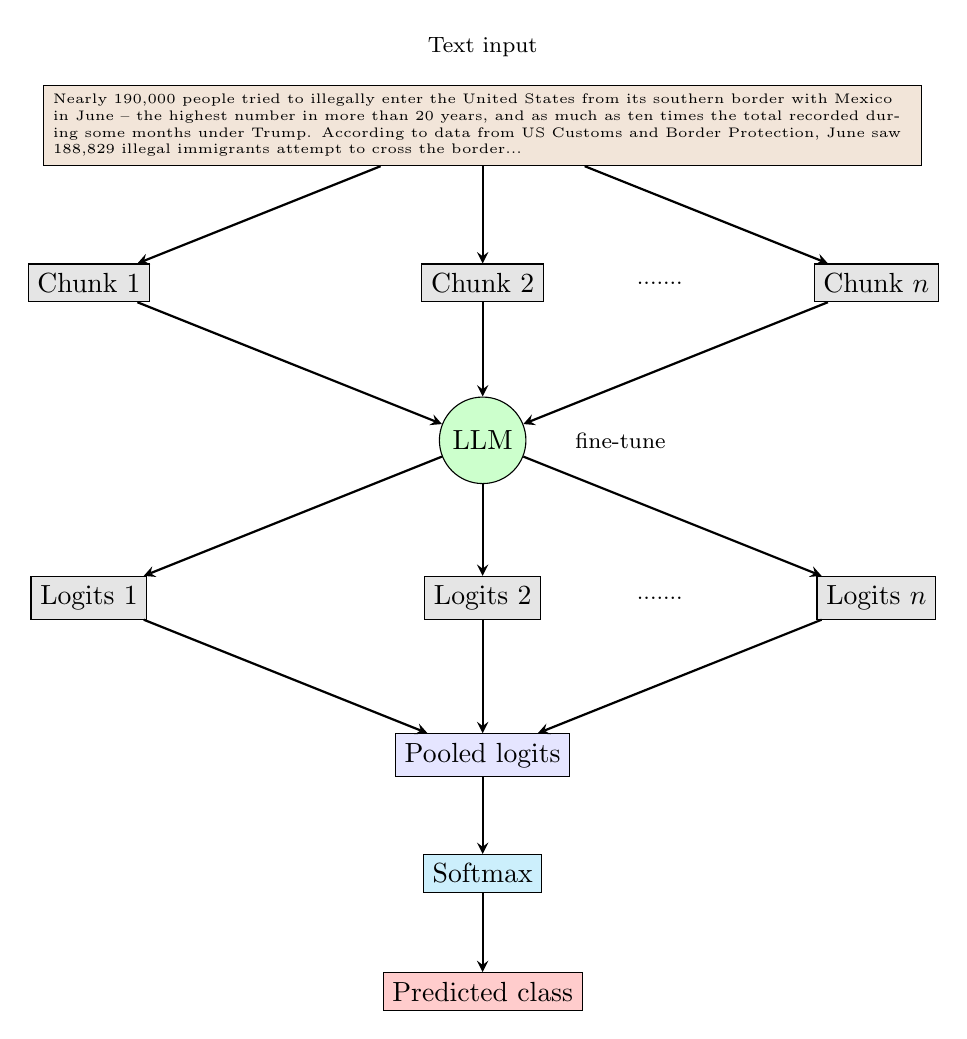
\begin{tikzpicture}
        \tikzstyle{arrow} = [thick,->,>=stealth]
        \tikzstyle{chunk} = [rectangle, draw, fill=gray!20]
        \tikzstyle{label} = [text centered,font=\footnotesize]

        \node[label] at (0, 1) {Text input};
        \node (input) [draw, align=left, text width=0.9\linewidth, font=\tiny, fill=brown!20] at (0, 0) {Nearly 190,000 people tried to illegally enter the United States from its southern border with Mexico in June – the highest number in more than 20 years, and as much as ten times the total recorded during some months under Trump. According to data from US Customs and Border Protection, June saw 188,829 illegal immigrants attempt to cross the border...};

        \node[chunk] (chunk1) [draw] at (-5, -2) {Chunk 1};
        \node[chunk] (chunk2) [draw] at (0, -2) {Chunk 2};
        \node[label] at (2.25, -2) {.......};
        \node[chunk] (chunk3) [draw] at (5, -2) {Chunk \(n\)};

        \draw[arrow] (input) -- (chunk1);
        \draw[arrow] (input) -- (chunk2);
        \draw[arrow] (input) -- (chunk3);

        \node (bert) [draw, circle, fill=green!20] at (0, -4) {LLM};
        \node[label] at (1.75, -4) {fine-tune};

        \draw[arrow] (chunk1) -- (bert);
        \draw[arrow] (chunk2) -- (bert);
        \draw[arrow] (chunk3) -- (bert);

        \node[chunk] (logits1) [draw] at (-5, -6) {Logits 1};
        \node[chunk] (logits2) [draw] at (0, -6) {Logits 2};
        \node[label] at (2.25, -6) {.......};
        \node[chunk] (logits3) [draw] at (5, -6) {Logits \(n\)};

        \draw[arrow] (bert) -- (logits1);
        \draw[arrow] (bert) -- (logits2);
        \draw[arrow] (bert) -- (logits3);

        \node (pooling) [draw, fill=blue!10] at (0, -8) {Pooled logits};

        \draw[arrow] (logits1) -- (pooling);
        \draw[arrow] (logits2) -- (pooling);
        \draw[arrow] (logits3) -- (pooling);

        \node (softmax) [draw, fill=cyan!20] at (0, -9.5) {Softmax};

        \draw[arrow] (pooling) -- (softmax);

        \node (pred) [draw, fill=red!20] at (0, -11) {Predicted class};

        \draw[arrow] (softmax) -- (pred);

    \end{tikzpicture}
    \caption{Chunked fine-tuning. The input article is split into chunks, each chunk is processed by the model as a mini batch, and the resulting logits are pooled before applying softmax operation.}
    \label{fig:chunk_bert_finetuning}
\end{figure}

Figure \ref{fig:chunk_bert_finetuning} illustrates the architecture of the chunked fine-tuning for LLMs. Input texts are tokenised and segmented into separate chunks containing parts of text input. Chunks have a fixed linear size, with the final chunk padded accordingly. A 'CLS' token is inserted at the beginning of each chunk, acting as a summary representation of the entire chunk sequence, and a 'SEP' token is inserted at the end of each chunk. Chunks are then stacked together and fed into the model as mini-batches for the fine-tuning process. The logits (output scores) produced by each chunk are then pooled together using mean pooling to produce the final logits. Finally, a softmax operation is applied to the final logits to obtain the class probabilities.

The chunking method bypasses the sequence length limitation of most LLMs such as BERT \cite{devlin-2019-bert}, allowing for full representation and processing of text input without any loss of information. In the implementation, a window size of 512 tokens is chosen with no overlap. Fine-tuning is conducted over 4 epochs using a weighted loss function, a learning rate of 2e-5, and 500 linear warm-up steps.

\subsection{Hierarchical transformer model}

\begin{figure}[htbp]
    \centering
    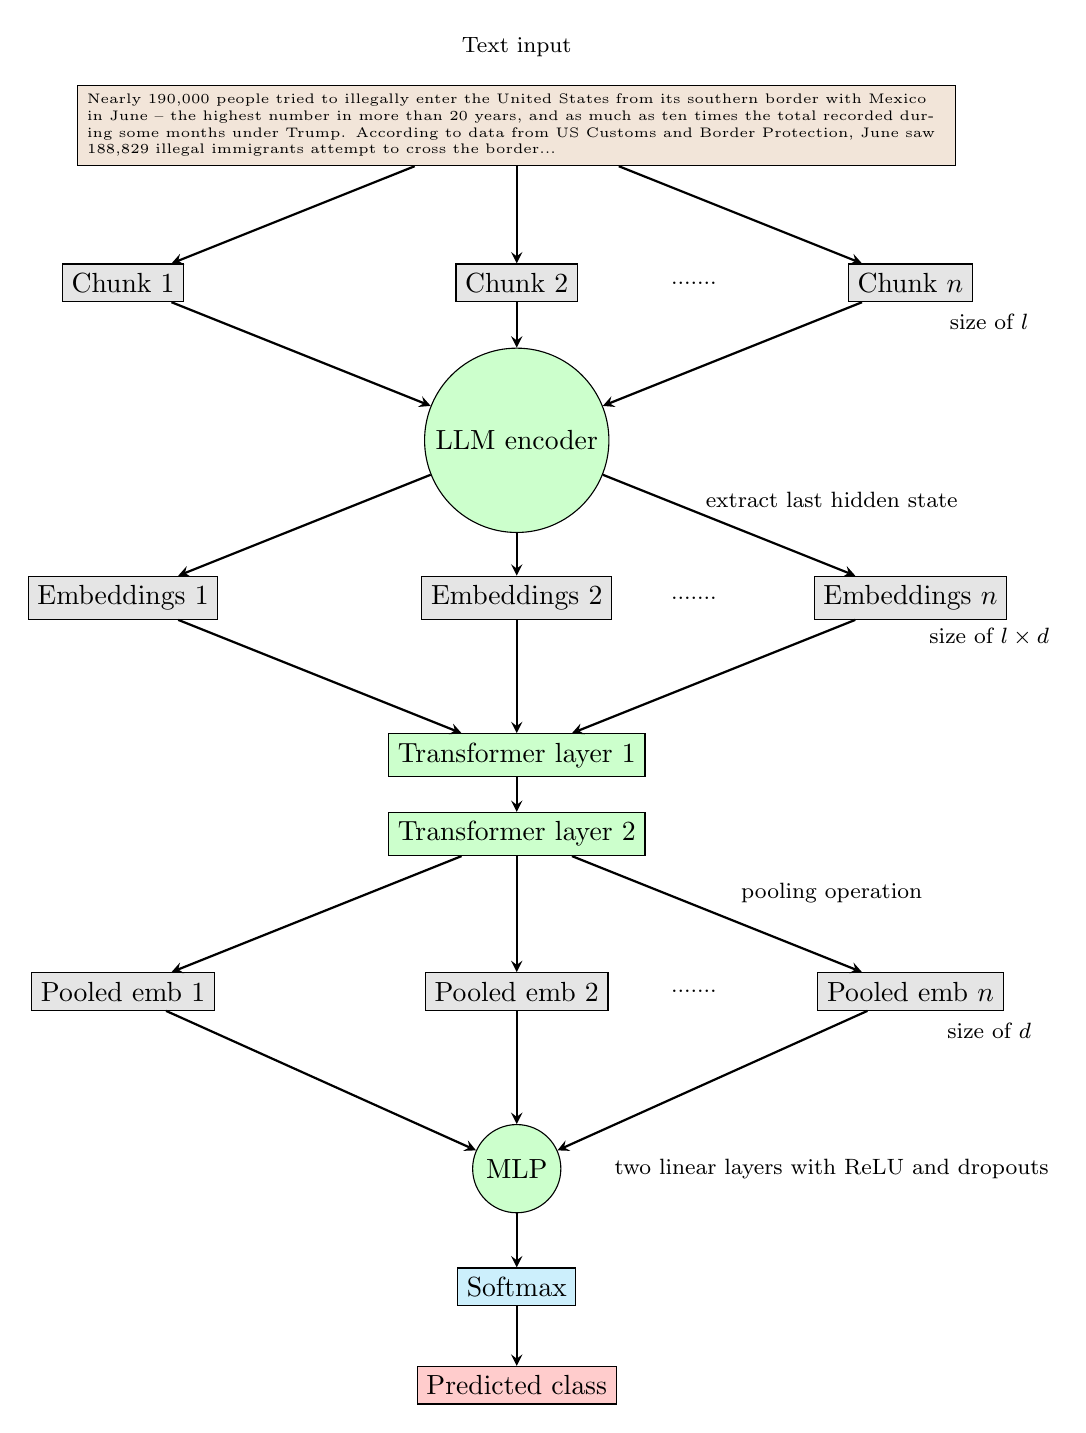
\begin{tikzpicture}
        \tikzstyle{arrow} = [thick,->,>=stealth]
        \tikzstyle{chunk} = [rectangle, draw, fill=gray!20]
        \tikzstyle{label} = [text centered, font=\footnotesize]

        \node[label] at (0, 1) {Text input};
        \node (input) [draw, align=left, text width=0.9\linewidth, font=\tiny, fill=brown!20] at (0, 0) {Nearly 190,000 people tried to illegally enter the United States from its southern border with Mexico in June – the highest number in more than 20 years, and as much as ten times the total recorded during some months under Trump. According to data from US Customs and Border Protection, June saw 188,829 illegal immigrants attempt to cross the border...};

        \node[chunk] (chunk1) [draw] at (-5, -2) {Chunk 1};
        \node[chunk] (chunk2) [draw] at (0, -2) {Chunk 2};
        \node[label] at (2.25, -2) {.......};
        \node[chunk] (chunk3) [draw] at (5, -2) {Chunk \(n\)};
        \node[label] at (6, -2.5) {size of \(l\)};

        \draw[arrow] (input) -- (chunk1);
        \draw[arrow] (input) -- (chunk2);
        \draw[arrow] (input) -- (chunk3);

        \node (encoder) [draw, circle, fill=green!20] at (0, -4) {LLM encoder};
        \node[label] at (4, -4.75) {extract last hidden state};

        \draw[arrow] (chunk1) -- (encoder);
        \draw[arrow] (chunk2) -- (encoder);
        \draw[arrow] (chunk3) -- (encoder);

        \node[chunk] (embedding1) [draw] at (-5, -6) {Embeddings 1};
        \node[chunk] (embedding2) [draw] at (0, -6) {Embeddings 2};
        \node[label] at (2.25, -6) {.......};
        \node[chunk] (embedding3) [draw] at (5, -6) {Embeddings \(n\)};
        \node[label] at (6, -6.5) {size of \( l \times d \)};

        \draw[arrow] (encoder) -- (embedding1);
        \draw[arrow] (encoder) -- (embedding2);
        \draw[arrow] (encoder) -- (embedding3);

        \node (tf_layer1) [draw, rectangle, fill=green!20] at (0, -8) {Transformer layer 1};

        \draw[arrow] (embedding1) -- (tf_layer1);
        \draw[arrow] (embedding2) -- (tf_layer1);
        \draw[arrow] (embedding3) -- (tf_layer1);

        \node (tf_layer2) [draw, rectangle, fill=green!20] at (0, -9) {Transformer layer 2};
        \draw[arrow] (tf_layer1) -- (tf_layer2);

        \node[label] at (4, -9.75) {pooling operation};

        \node[chunk] (pooled1) [draw] at (-5, -11) {Pooled emb 1};
        \node[chunk] (pooled2) [draw] at (0, -11) {Pooled emb 2};
        \node[label] at (2.25, -11) {.......};
        \node[chunk] (pooled3) [draw] at (5, -11) {Pooled emb \(n\)};
        \node[label] at (6, -11.5) {size of \(d\)};

        \draw[arrow] (tf_layer2) -- (pooled1);
        \draw[arrow] (tf_layer2) -- (pooled2);
        \draw[arrow] (tf_layer2) -- (pooled3);

        \node (mlp) [draw, circle, fill=green!20] at (0, -13.25) {MLP};
        \node[label] at (4, -13.25) {two linear layers with ReLU and dropouts};

        \draw[arrow] (pooled1) -- (mlp);
        \draw[arrow] (pooled2) -- (mlp);
        \draw[arrow] (pooled3) -- (mlp);

        \node (softmax) [draw, fill=cyan!20] at (0, -14.75) {Softmax};

        \draw[arrow] (mlp) -- (softmax);

        \node (pred) [draw, fill=red!20] at (0, -16) {Predicted class};

        \draw[arrow] (softmax) -- (pred);
    \end{tikzpicture}
    \caption{CLS method architecture}
    \label{fig:cls_method}
\end{figure}


Figure \ref{fig:cls_method} shows the full architecture of the hierarchical transformer model, similarly implemented by Su et al. \cite{su-2021-classifying} for classifying long clinical documents. This method begins by similarly segmenting the input text into smaller chunks. These chunks are encoded into a higher dimensional feature space by feeding them into a pre-trained Large Language Model (LLM) and extracting the last hidden state, also known as \textit{feature-based approach} as described in \cite{sun-2020-fine-tune}. Subsequently, the encoded chunks are then passed into two transformer layers. Afterwards, each chunk is pooled together, resulting in embedding of size \(d\), serving as a concise summary of the entire chunk sequence. This summary representation is then processed through a Multi-Layer Perceptron (MLP). Lastly, a softmax operation will be applied to the output of the MLP layer to determine the final output class.

Two different pre-trained models are experimented as the LLM encoder in this method: BERT \cite{devlin-2019-bert} and MAGPIE \cite{horych-2024-magpie}. The MLP consists of two linear layers with ReLU activation function \cite{agarap-2018-relu} and dropouts. Chunk size is set to 156 tokens, two transformer layers are used, and 0.2 probability is applied to the dropout layer. Training is done over 3 epochs with weighted loss, 1e-5 learning rate and 162 warm-up steps (10\% of total training steps).

\section{Training details}

All methods are implemented in Python 3.12.0 \cite{van-1995-python} using the PyTorch \cite{paszke-2017-pytorch} and transformers \cite{wolf-2020-huggingface} package from HuggingFace. The BERT model utilised in these methods is the 'bert-base-cased' instead of the 'bert-base-uncased' to account for distinctions in capitalised words, which may be crucial \cite{devlin-2019-bert}. The AdamW \cite{loshchilov-2019-adamw} optimiser and Cross Entropy Loss is used in all cases. The batch size is set to 8 for all deep learning methods.

\subsection{Weighted loss}

Weighted loss addresses the problem of training models on an imbalanced dataset by assigning higher weights to classes with fewer instances and lower weights to classes with more instances. This adjustment ensures that the model pays more attention to correctly predicting the minority class, thereby improving overall performance metrics. Using weighted loss during training is preferred over oversampling the minority class. Oversampling can generate synthetic examples that may not accurately represent real-world articles, potentially leading to less robust model performance \cite{alkhawaldeh-2023-challenges}. Additionally, undersampling is also not ideal due to the small size of the dataset and the significant disparity between the majority and minority classes. The weighted loss is gained by calculating class weights (as seen in Figure \ref{fig:class_weights}) through the scikit-learn library \cite{pedregosa-2011-scikit-learn}, which are then inserted into the loss function.

\begin{figure}[htbp]
    \centering
    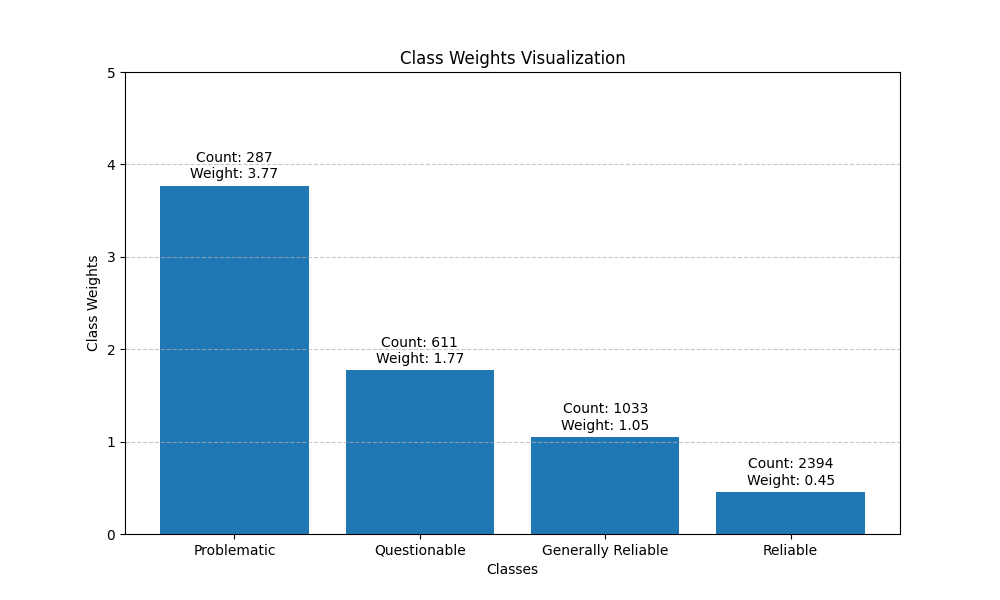
\includegraphics[width=0.9\linewidth]{figures/class_weights.png}
    \caption{Class weights in the training set}
    \label{fig:class_weights}
\end{figure}



%%% Local Variables: 
%%% mode: latex
%%% TeX-master: "thesis"
%%% End: 
